\begin{trapbox}
  \textbf{\textcolor{CTrap}{易错点一｜把“横坐标乘 $2$”写成 $f(2x)$}}
  \textbf{错误：} 横坐标变为 $2$ 倍，就写成 $y=f(2x)$。\\
  \textbf{正确：} 横坐标乘 $2$ 时应写成 $y=f(x/2)$。以 $f(x)=x^2$ 为例，原点 $(2,4)$ 应移到 $(4,4)$，而不是 $(1,4)$。
  \begin{center}
  \begin{tikzpicture}[x=1.18cm,y=0.72cm,>=stealth,every node/.style={font=\small}]
    \draw[->,gray!75] (-0.2,0)--(4.8,0) node[below] {$x$};
    \foreach \x in {1,2,3,4}{\draw (\x,0.08)--(\x,-0.08) node[below] {$\x$};}
    \draw[densely dashed,gray!65] (0,1.15)--(4.45,1.15);
    \fill[red!75!black] (1,1.15) circle (2.2pt) node[above,yshift=15pt] {错：$(1,4)$};
    \fill[blue!75!black] (2,1.15) circle (2.2pt) node[above] {原：$(2,4)$};
    \fill[orange!85!black] (4,1.15) circle (2.2pt) node[above] {对：$(4,4)$};
    \draw[->,thick,orange!85!black] (2.13,0.91)--(3.86,0.91);
  \end{tikzpicture}

  \end{center}
  \textbf{自检：} 先算一个点移到哪里，再看新解析式是否经过它。

  \medskip
  \textbf{\textcolor{CTrap}{易错点二｜看见“乘 $2$”就以为图像变宽}}
  \textbf{错误：} $f(2x)$ 比 $f(x)$ 宽。\\
  \textbf{正确：} $f(2x)$ 的横坐标实际变为原来的 $1/2$，所以\textbf{变窄}；$f(x/2)$ 才是\textbf{变宽 $2$ 倍}。
  \begin{center}
  \begin{tikzpicture}[x=1cm,y=0.39cm,>=stealth,every node/.style={font=\small}]
    \draw[->,gray!75] (-4.1,0)--(4.2,0) node[below] {$x$};
    \draw[->,gray!75] (0,-0.25)--(0,4.7) node[left] {$y$};
    \draw[orange!85!black,very thick,domain=-1.05:1.05,samples=65] plot (\x,{4*\x*\x});
    \draw[blue!75!black,thick,domain=-2.08:2.08,samples=65] plot (\x,{\x*\x});
    \draw[green!55!black,very thick,domain=-4:4,samples=65] plot (\x,{\x*\x/4});
    \node[orange!85!black,anchor=west] at (4.7,4.5) {$f(2x)$ 窄};
    \node[blue!75!black,anchor=west] at (4.7,2.5) {$f(x)$};
    \node[green!55!black,anchor=west] at (4.7,.5) {$f(x/2)$ 宽};
  \end{tikzpicture}

  \end{center}
  \textbf{口诀：} “里面乘大，图变窄；里面乘小，图变宽。”此处说的是\textbf{乘正数}。

  \medskip
  \textbf{\textcolor{CTrap}{易错点三｜漏看 $\omega=1$ 或定义域}}
  \textbf{错误：} 以为 $\omega=1$ 时也会变宽或变窄；或者认为新函数可以代入任何 $x$。\\
  \textbf{正确：} $f(1\cdot x)=f(x)$，\textbf{图像原样不动}；如果是 $\ln(x/2)$，仍必须满足 $x>0$。
  \begin{center}
  \begin{tikzpicture}[x=1.02cm,y=0.58cm,>=stealth,every node/.style={font=\small}]
    \draw[->,gray!75] (-1.95,0)--(2.0,0) node[below] {$x$};
    \draw[->,gray!75] (0,-0.2)--(0,3.1) node[left] {$y$};
    \draw[very thick,blue!75!black,domain=-1.7:1.7,samples=65] plot (\x,{\x*\x});
    \draw[orange!85!black,densely dashed,thick,domain=-1.7:1.7,samples=65] plot (\x,{\x*\x});
    \fill[orange!85!black] (1,1) circle (2.3pt);
    \node[right] at (1.05,1.1) {$(1,1)$ 不动};
    \node[align=left,above] at (0,3.1) {$f(x)$ 与 $f(1x)$ 完全重合};
  \end{tikzpicture}

  \end{center}
  \textbf{自检：} 先看系数是否等于 $1$；再检查原函数的输入范围。

  \medskip
  \textbf{\textcolor{CTrap}{易错点四｜横向平移、横向伸缩的顺序弄反}}
  \textbf{对比：} 从 $y=x^2$ 出发：
  \begin{itemize}[leftmargin=*,itemsep=0.2em,topsep=0.2em]
    \item \textbf{先向右平移 $1$，再横向压成 $1/2$：} $y=(x-1)^2\to (2x-1)^2$，最低点的横坐标为 $1/2$。
    \item \textbf{先横向压成 $1/2$，再向右平移 $1$：} $y=4x^2\to 4(x-1)^2$，最低点的横坐标为 $1$。
  \end{itemize}
  \begin{center}
  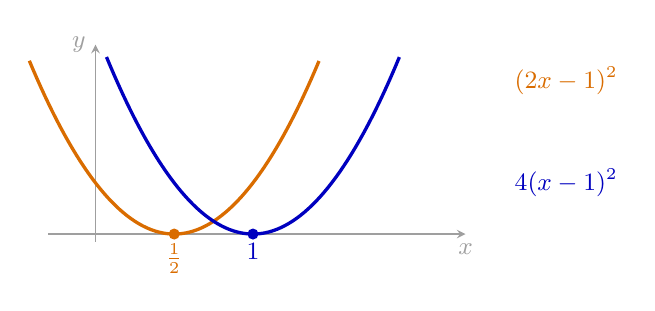
\begin{tikzpicture}[x=2cm,y=0.65cm,>=stealth,every node/.style={font=\small}]
    \draw[->,gray!75] (-0.3,0)--(2.35,0) node[below] {$x$};
    \draw[->,gray!75] (0,-0.15)--(0,3.7) node[left] {$y$};
    \draw[very thick,orange!85!black,domain=-0.42:1.42,samples=75] plot (\x,{(2*\x-1)^2});
    \draw[very thick,blue!75!black,domain=0.07:1.93,samples=75] plot (\x,{4*(\x-1)^2});
    \fill[orange!85!black] (0.5,0) circle (2pt);
    \fill[blue!75!black] (1,0) circle (2pt);
    \node[below,orange!85!black] at (0.5,0) {$\frac12$};
    \node[below,blue!75!black] at (1,0) {$1$};
    \node[orange!85!black,anchor=west] at (2.6,3) {$(2x-1)^2$};
    \node[blue!75!black,anchor=west] at (2.6,1) {$4(x-1)^2$};
  \end{tikzpicture}

  \end{center}
  \textbf{记住：} \textbf{每做一步，就先写出当时的解析式。} 横向平移和横向伸缩通常不能换序；\textbf{向上平移和横向伸缩}在本结论条件下可以换序。
\end{trapbox}
